\subsection{Glyph: \glyph{Positive influence}}
\label{sec:af:positive_infl}

In \SBGNAFLone, a \emph{positive influence} is defined as an action that produces positive or activating effect from one activity to another.

\begin{glyphDescription}

\glyphSboTerm SBO:0000170 ! stimulation

 \glyphOrigin Any \glyph{Activity node} (\sect{af:ANs}) or any \glyph{logical operator} (\sect{af:logic}).
 \glyphTarget Any \glyph{biological activity} or \glyph{phenotype} (\sect{af:ANs}).
 \glyphEndPoint The target extremity of a \glyph{positive influence} carries an open arrow pointing to the target activity node (\fig{af:positiveInfl}).

\end{glyphDescription}

\begin{figure}[H]
  \centering
  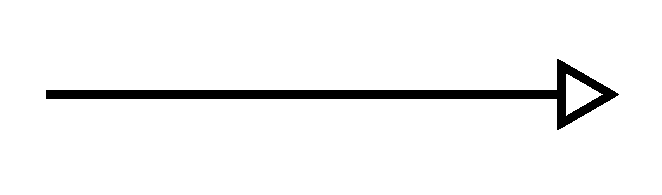
\includegraphics[width = 2in]{images/positiveInfluence}
  \caption{The \AF glyph for \glyph{positive influence}.}
  \label{fig:af:positiveInfl}
\end{figure}

\begin{figure}[H]
  \centering
  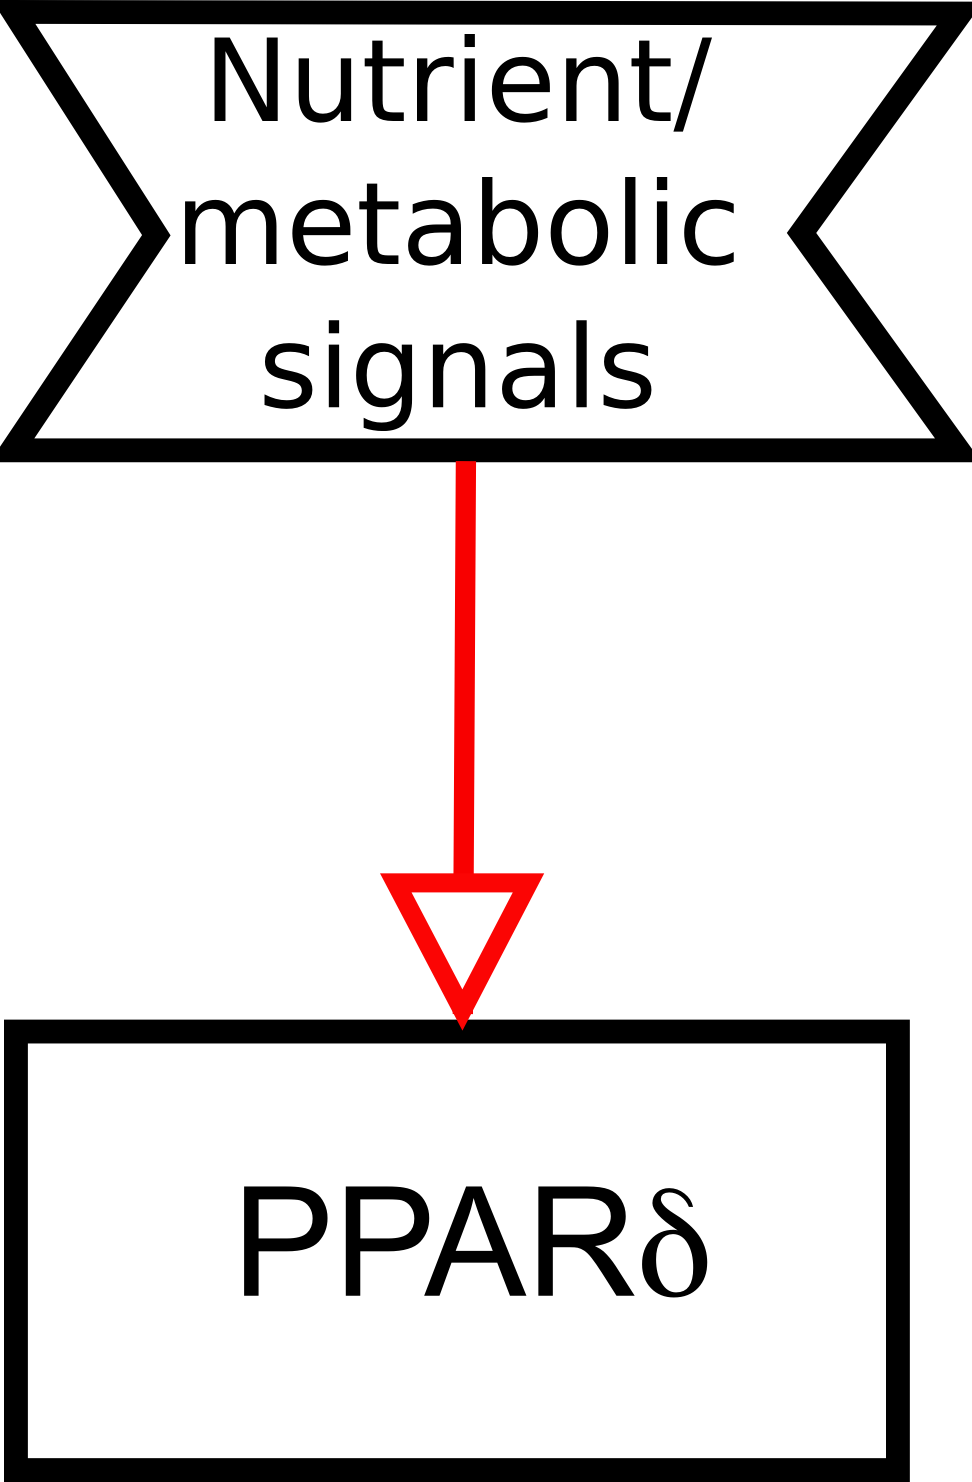
\includegraphics[width = 2in]{examples/ex-positiveInfluence}
  \caption{An exmaple of \glyph{positive influence} from a \glyph{perturbation} to the to the nuclear hormone receptor PPAR$\delta$.}
  \label{fig:af:exPI}
\end{figure} 